% !TEX root = ../main.tex
\subsection{Validation and Results}
\label{12.40::validation_and_results}
% --+ Data used +---------------------------------------------------------------
    Just like the residuals validation, the results presented in this document are based on the application of this work to RG-F data.
    It is important to note that the RG-F target is approximately 55 centimetres long, which is much larger than the average CLAS12 target \cite{hattawy2019}.
    Specifically, the runs used for testing and validation are presented in Table \ref{tab::12.40::rgf_data}, and the run used to obtain the data displayed in this section was 011983.

    \begin{table}[h!]
        \centering
        \begin{tabular}{lllll}
            \toprule
            \textbf{Run Number} & \textbf{Energy (MeV)} & \textbf{Current (nA)} & \textbf{Configuration} & \textbf{Target} \\
            \midrule \midrule
            011983              & 10389.4               &  50                   & Inbending              & D2 \\
            012016              & 10389.4               & 250                   & Inbending              & D2 \\
            012439              &  2186.4               &  15                   & Inbending              & H2 \\
            012461              & 10196.6               &  20                   & Inbending              & D2 \\
            \bottomrule
        \end{tabular}
        \caption{RG-F runs used for validation.}
        \label{tab::12.40::rgf_data}
    \end{table}

    % !TEX root = ../main.tex
\subsubsection{Cuts}
\label{12.41::cuts}
    \begin{figure}[b!]
        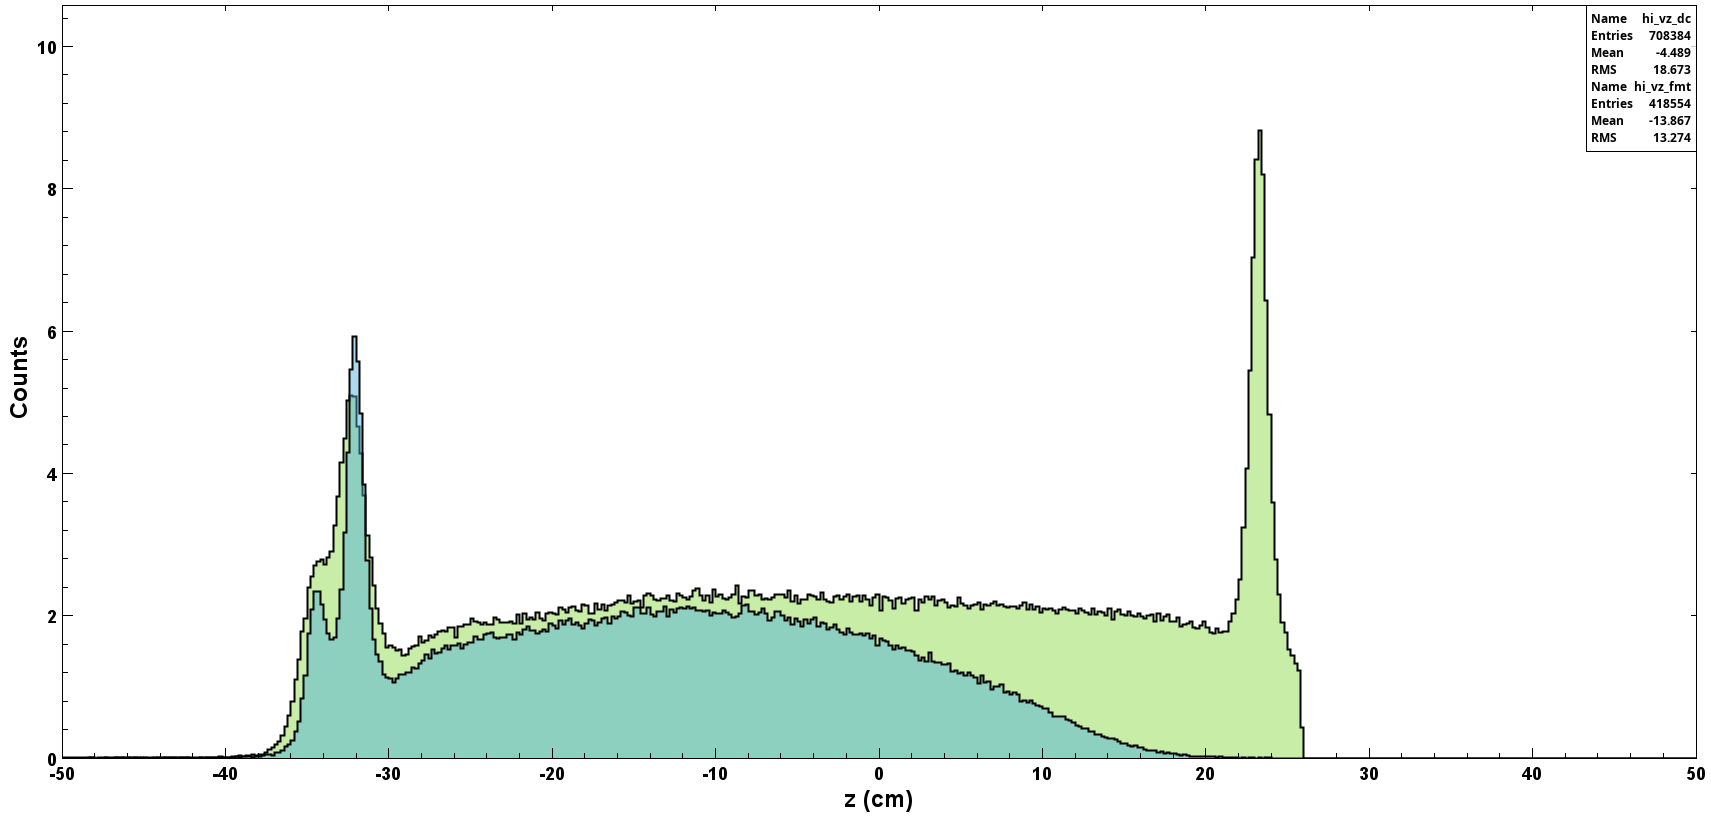
\includegraphics[width=\textwidth]{41dc_vs_fmt.png}
        \caption[DC vs. FMT $z$ without geometric correction]
        {DC vs. FMT vertex $z$ for electrons without any geometric correction.
        DC tracks are shown in green while FMT tracks are shown in blue.
        Note that the dark cyan colour comes from the overlap.}
        \floatfoot{Source: Own elaboration, using the \texttt{fmtVertex.groovy} script in \href{https://github.com/JeffersonLab/clas12alignment}{CLAS12 alignment software}.}
        \label{fig::12.41::dc_vs_fmt_vz_11983}
    \end{figure}

    Some additional cuts are applied to the tracks to obtain the plots presented in this section.
    These cuts are used to remove very poor tracks that would not be suitable for analysis regardless.
    The applied cuts are as follows:
    \begin{itemize}
        \item
            \texttt{abs(chi2pid) < 5}:
            This cut removes tracks that do not provide sufficient certainty regarding the particle's PID.
        \item
            \texttt{vz < fmtZ}:
            This cut removes tracks located further downstream than the FMT.
        \item
            \texttt{chi2/ndf < 15}:
            This cut excludes tracks with excessively high uncertainty.
    \end{itemize}

    % !TEX root = ../main.tex
\subsubsection{Geometry Effect}
\label{12.42::geometry_effect}
    To evaluate the enhancement in vertex resolution, we will compare the vertex positions of tracks that underwent only DC reconstruction with those that underwent both DC and FMT reconstruction.
    For convenience, we will refer to the former as DC tracks and the latter as FMT tracks.
    Considering that the $z$ axis is aligned with the beamline, Figure \ref{fig::12.41::dc_vs_fmt_vz_11983} illustrates the $z$ positions of the vertex for DC tracks versus FMT tracks.

    To comprehend the plot in Figure \ref{fig::12.41::dc_vs_fmt_vz_11983}, it is valuable to examine the RG-F target.
    The target consists of a large gas-filled chamber with a varying composition across different runs.
    The distance between the chamber windows measures $553.32$ millimetres.
    Furthermore, it was observed that the upstream window of the target is positioned approximately $24$ millimetres away from the beam window.
    All windows are constructed from aluminium and have a thickness of $15$ micrometers.
    A detailed depiction of the target can be found in Addendum 1.

    Based on Figure \ref{fig::12.41::dc_vs_fmt_vz_11983}, it is evident that the FMT detector solely detects the upstream windows, completely overlooking the downstream one.
    This issue stems from a geometric constraint: the downstream window falls outside the active detection area of the FMT.
    This effect is clearly illustrated in Figure \ref{eq::12.42::vz_vs_theta}, where the $\theta$ angle is plotted against the vertex $z$ coordinate.
    The two red lines in the plots represent the FMT's active area, and it is apparent that the downstream window lies outside this region, thereby explaining its absence.

    \begin{figure}[t!]
        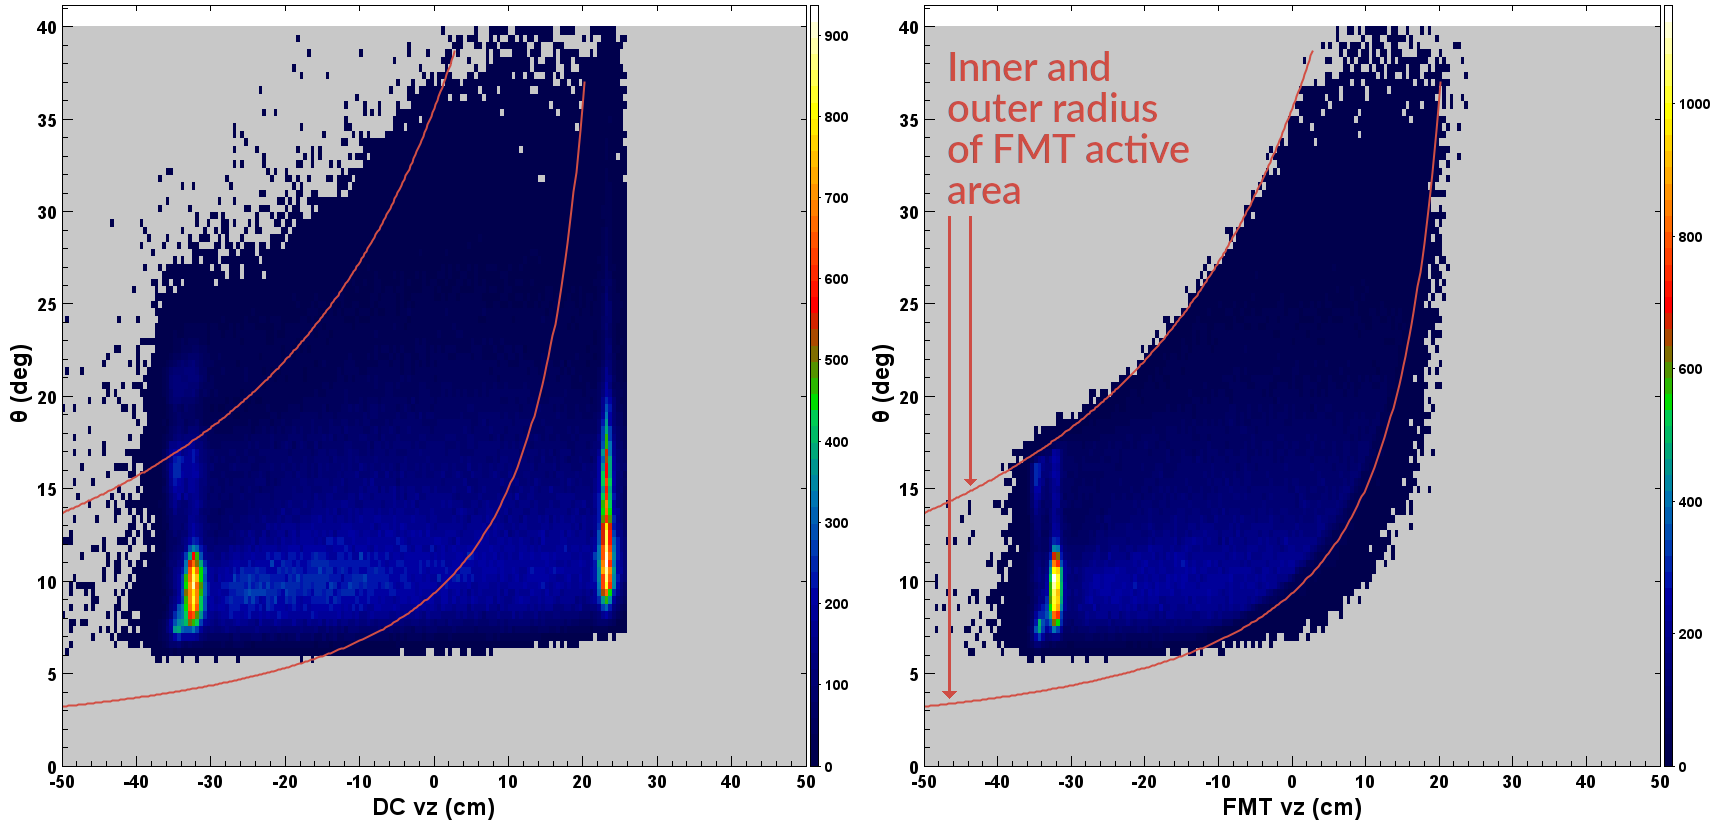
\includegraphics[scale=0.24]{42theta_dc_vs_fmt.png}
        \caption[$z$ vs. $\theta$ for DC and FMT]
        {$z$ vs. $\theta$ for DC and FMT for electrons without any geometry correction.
        FMT's active area are shown in red lines.}
        \floatfoot{Source: Own elaboration, using the \texttt{fmtVertex.groovy} script in \href{https://github.com/JeffersonLab/clas12alignment}{CLAS12 alignment software}.}
        \label{eq::12.42::vz_vs_theta}
    \end{figure}

    To compensate for this geometric effect, we introduce an additional cut based on the plotted curves.
    The curves can be described by the following equations
    \begin{equation}
        c_1(z) = 57.29 \cdot \arctan\left(\frac{r_\text{inner}}{z_0 - z}\right),
        \hspace{0.5cm}
        c_2(z) = 57.29 \cdot \arctan\left(\frac{r_\text{outer}}{z_0 - z}\right).
        \label{eq::12.42::fmt_geometry_cut}
    \end{equation}

    Here, $r_\text{inner}$ represents the radius of the hole at the center of the FMT, $r_\text{outer}$ denotes the radius of the outer circumference of the FMT, and $z_0$ corresponds to the $z$ position of the first FMT layer plus the drift distance.
    All these parameters are obtained from the CCDB.

    % !TEX root = ../main.tex
\subsubsection{Vertex Resolution Improvement}
\label{12.43::vertex_resolution_improvement}

    \begin{figure}[b!]
        \frame{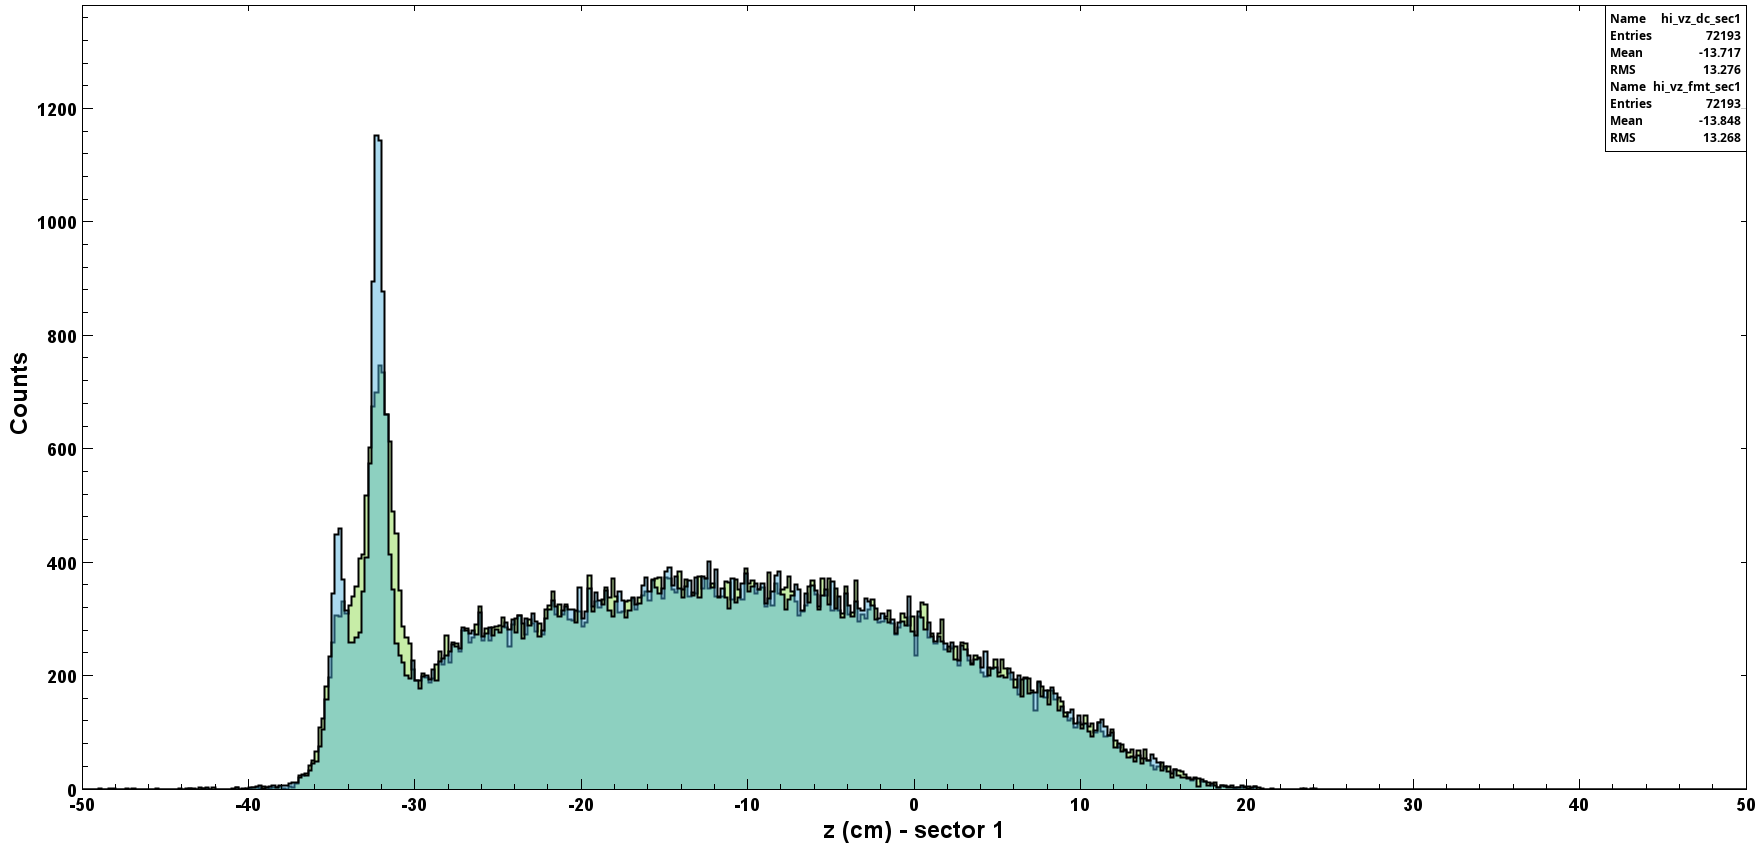
\includegraphics[scale=0.24]{40dc_vs_fmt_sector1.png}}
        \caption[DC vs FMT $z$ with geometry correction]
        {DC vs FMT vertex $z$ for electrons with a geometric correction.
        DC tracks are shown in green while FMT tracks are shown in blue.
        Data from only one CLAS12 sector was used to obtain this plot.}
        \floatfoot{Source: Own elaboration, using the \texttt{fmtVertex.groovy} script in \href{https://github.com/JeffersonLab/clas12alignment}{CLAS12 alignment software}.}
        \label{fig::12.43::dc_vs_fmt_vz_11983_corrected}
    \end{figure}

    Furthermore, an additional cut has been introduced.
    As of the FMT alignment work, beam alignment for RG-F data had not been carried out, resulting in a decrease in vertex resolution.
    To mitigate the impact of this alignment issue on reconstruction accuracy, we have implemented a cut to utilise only one sector of the detector.

    The resolution plot, comparing DC and FMT tracks after applying all the previously mentioned cuts, is depicted in Figure \ref{fig::12.43::dc_vs_fmt_vz_11983_corrected}.
    To evaluate the resolution for both DC and FMT tracks, we utilise a fit consisting of two Gaussian curves combined with a quadratic curve to account for the background.
    The fit is defined as follows
    \begin{equation*}
        \text{amp}_1 \cdot \text{gaus}(z, z_\text{max}, \sigma) + \text{amp}_2 \cdot \text{gaus}(z, z_\text{max} - 2.4, \sigma) + p_1 + p_2\cdot z + p_3\cdot z^2,
    \end{equation*}
    where
    \begin{itemize}
        \item
            $\text{amp}1$ represents the amplitude of the largest peak, and $z\text{max}$ corresponds to its $z$ position,
        \item
            $\text{amp}_2$ signifies the amplitude of the leftward peak, which has been measured to be at a position of $2.4$ centimetres, and
        \item
            the remaining parameters, $p_1$, $p_2$, and $p_3$, are obtained through the fitting process.
    \end{itemize}

% --+ Resolution for electrons +------------------------------------------------
    For electrons in run 011983 (low luminosity, 50 nA), the analysis yields a DC resolution of $\sigma_\text{DC} = 0.875$ cm and an FMT resolution of $\sigma_\text{FMT} = 0.387$ cm.
    This indicates a doubling of the resolution achieved with the inclusion of the FMT detector.

    Similarly, for electrons in run 012016 (production luminosity, $250$ nA), the analysis shows a DC resolution of $\sigma_\text{DC} = 1.009$ cm and an FMT resolution of $\sigma_\text{FMT} = 0.596$ cm.

    % !TEX root = ../main.tex
\subsubsection{Conclusions}
\label{12.44::conclusions}
    Although the improvement in resolution is not as significant as initially anticipated for the detector, it remains an encouraging result.
    The enhanced resolution enables more precise measurements of the target position.
    As a practical implication, it allows for double targets to be positioned closer to each other, thereby benefiting the derived physics from experiments like the RG-E run.

    The reason for the smaller-than-predicted improvement in resolution can be attributed to the initial projection, which assumed the presence of six FMT layers.
    The inclusion of six layers would provide additional positional data along the particle's track, thereby enhancing the accuracy of the vertex position measurement during the fitting process.

% --+ Why no improvements is seen on vertex momentum resolution +---------------
    Furthermore, due to the limited number of layers and their close proximity in the FMT detector, it exhibits a small lever arm.
    As a result, the detector's contribution to the vertex momentum resolution is not significant, as it does not provide sufficient additional data to accurately determine the track's momentum.

% --+ Show detector efficiency +------------------------------------------------
    In order to gain a better understanding of the FMT detector, we conducted a brief study on its efficiency.
    The efficiency is defined as the ratio of the number of FMT tracks to the number of DC tracks, representing how many of the DC tracks were also detected by the FMT.

    For the three-layer configuration, the efficiency is approximately $88.96\%$.
    Figure \ref{fig::12.44::fmt_azimuthal_efficiency} illustrates the layer-by-layer efficiency, showing no anomalous geometric effects.
    The observed gaps in efficiency are solely a result of the CLAS12 detector's geometry, which is divided into six sectors.

    \begin{figure}[b]
        \centering\frame{
        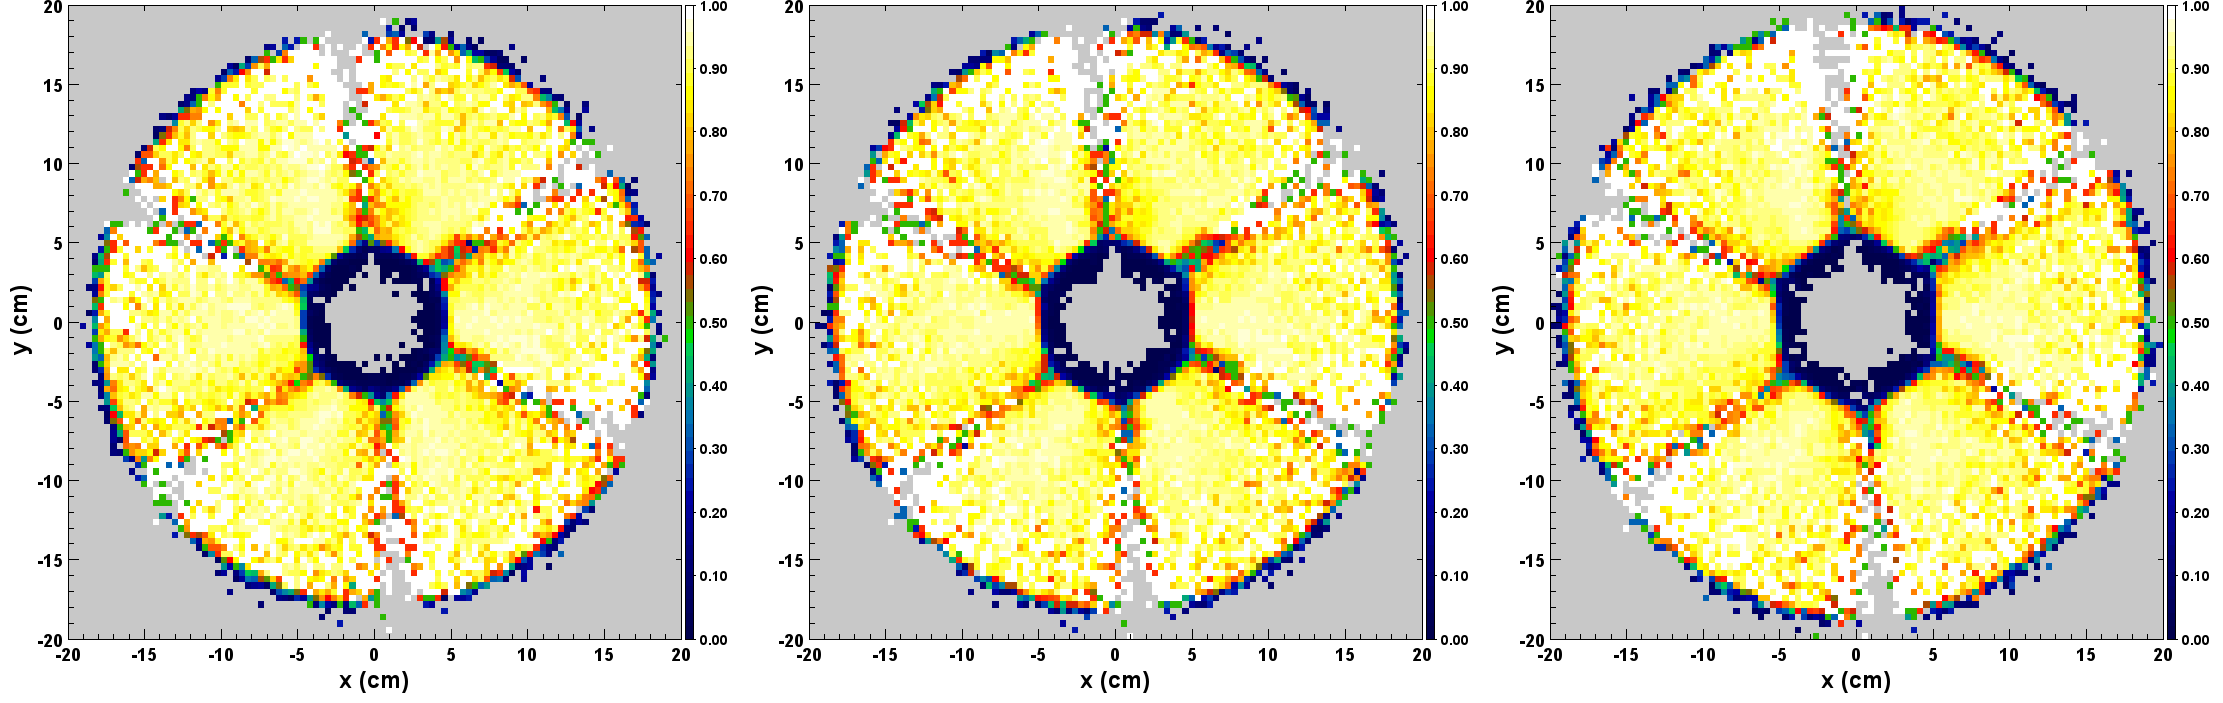
\includegraphics[width=\textwidth]{44fmt_efficiency.png}}
        \caption[FMT layers efficiency]{Efficiency of each FMT layer.
        Source: \texttt{fmtVertex.groovy} script in \hyperlink{github.com/JeffersonLab/clas12alignment}{CLAS12 alignment software}.}
        \label{fig::12.44::fmt_azimuthal_efficiency}
    \end{figure}

